\documentclass[11pt, a4paper, oneside]{article} 
% use "amsart" instead of "article" for AMSLaTeX format
%\usepackage{mydefs,mythm}
\usepackage[textsize=footnotesize,textwidth=3cm]{todonotes}
% \geometry{landscape} % Activate for rotated page geometry
% \usepackage[parfill]{parskip} % Activate to begin paragraphs with an empty line rather than an indent

\newcommand{\Lam}{\Lambda}
\newcommand{\Lamc}{{\bar{\Lambda}}}
\usepackage{amsthm}
\newtheorem{thm}{Theorem}
\newtheorem{theorem}[thm]{Theorem}
\newtheorem{conj}[thm]{Conjecture}
\newtheorem{conjecture}[thm]{Conjecture}
\newtheorem{cor}[thm]{Corollary}
\newtheorem{corollary}[thm]{Corollary}
\newtheorem{lem}[thm]{Lemma}
\newtheorem{lemma}[thm]{Lemma}
\newtheorem{prop}[thm]{Proposition}
\newtheorem{proposition}[thm]{Proposition}

\newtheorem{ax}{Axiom}
\newtheorem{axiom}{Axiom}
\newtheorem{claim}{Claim}
\theoremstyle{definition}
\newtheorem{defn}{Definition}
\newtheorem{definition}{Definition}
\newtheorem{ex}{Example}
\newtheorem{example}{Example}
\theoremstyle{remark}
\newtheorem{notation}{Notation}
\newtheorem{remark}{Remark}
\newtheorem{rem}{Remark}

\PassOptionsToPackage{override}{xcolor} % Beamer option
\usepackage[utf8]{inputenc}
\usepackage{hyperref}
\usepackage{subfig}
\usepackage{amsmath} 
\usepackage{amssymb}
\usepackage{amsfonts,amssymb}
\usepackage{dsfont}
\usepackage[mathscr]{euscript}
\usepackage{enumerate,xspace,threeparttable}
\usepackage{graphicx}
\usepackage{verbatim}
\usepackage{algorithmic}
\usepackage{listings}
\usepackage{wrapfig}
\usepackage{translator}

\providecommand{\ie}{i.e.\ }
\providecommand{\qr}{\eqref}
\renewcommand{\d}{\,d}
\providecommand{\dd}[2]{\dfrac{d#1}{d#2}}
\providecommand{\qtext}[1]{\quad\text{#1}\quad}

\providecommand{\RR}{\mathbb{R}}
\providecommand{\CC}{\mathbb{C}}
\providecommand{\TT}{\mathbb{T}}
\providecommand{\ZZ}{\mathbb{Z}}
\providecommand{\QQ}{\mathbb{Q}}
\providecommand{\NN}{\mathbb{N}}
\providecommand{\VV}{\mathbb{V}}
\providecommand{\PP}{\mathsf{P}}
\providecommand{\EE}{\mathsf{E}}
\providecommand{\BB}{\mathbb{B}}
\renewcommand{\SS}{\mathbb{S}}

\providecommand{\CF}{\mathscr{F}}
\providecommand{\CB}{\mathscr{B}}
\providecommand{\CA}{\mathscr{A}}
\providecommand{\CR}{\mathscr{R}}
\providecommand{\CH}{\mathscr{H}}
\providecommand{\CM}{\mathscr{M}}
\providecommand{\CT}{\mathscr{T}}

\providecommand{\mfrak}{\mathfrak}
\providecommand{\mscr}{\mathscr}
\providecommand{\mc}{\mathcal}
\providecommand{\mb}{\mathbf}
\providecommand{\bs}{\boldsymbol}
\providecommand{\mbb}{\mathbb}
\providecommand{\ms}{\mathsf}
\providecommand{\vv}[2]{\ensuremath{\overrightarrow{#1#2}}} % vector
\providecommand{\opn}{\operatorname}
\providecommand{\ol}{\overline}
\def\ii#1{^{(#1)}}
\providecommand{\E}{\mathsf{E}}
\renewcommand{\P}{\mathsf{P}}
\renewcommand{\Pr}[1]{\P\left(#1\right)}
\providecommand{\Ex}[1]{\E(#1)}

\providecommand{\Var}{\opn{Var}}
\providecommand{\var}{\opn{var}} 
\providecommand{\Cov}{\opn{Cov}}
\providecommand{\sign}{\opn{sign}}
\providecommand{\diag}{\opn{diag}}

\providecommand{\msf}{\mathsf}
\providecommand{\ett}{\mathsf{1}}

\providecommand{\Ordo}[1]{{O(#1)}} 
\providecommand{\ordo}[1]{{o(#1)}} 
\providecommand{\OrdoOmega}[1]{{\varOmega(#1)}} 
\providecommand{\OrdoTheta}[1]{\ensuremath{\Theta(#1)}} 
\providecommand{\ordoomega}[1]{\ensuremath{\omega(#1)}}

\providecommand{\e}{\epsilon}
\providecommand{\tl}{\tilde}
\providecommand{\g}{\gamma}
\providecommand{\w}{\omega}
\providecommand{\C}{C}
\providecommand{\scp}[2]{\ensuremath{\left\langle#1,#2\right\rangle}}

\providecommand{\bmat}[1]{\begin{bmatrix} #1 \end{bmatrix}}
\providecommand{\T}{^{\!\mathrm{T}}}
\providecommand{\ds}{\displaystyle}

\renewcommand{\L}{\mathscr{L}}

\def\Ex#1{\EE\left[#1\right]}

\def\dom{\opn{dom}}

\def\X{\mscr X}
\def\T{\opn{\msf{T}}}


\def\ilim{\varinjlim}
\def\plim{\varprojlim}
\def\lover#1{\overset{#1}{\longleftarrow}}
\def\rover#1{\overset{#1}{\longrightarrow}} 
\def\npair#1#2{\left\langle\, #1\mid #2\,\right\rangle}
\def\F{\mscr F}

\def\scp#1#2{\left\langle #1 , #2 \right\rangle}

\title{Existence for an eigenfunction for the critical phase of the Dyson model}

\author{Anders Johansson and Anders \"Oberg}
\date{}
\begin{document}
\maketitle


\section{Introduction}\noindent
It is well-known that there exists a continuous and strictly positive
eigenfunction $h$ for any transfer operator defined on a symbolic shift space
with finitely many symbols such that the potential has summable variations. Here
we prove the existence of an eigenfunction for the important special class of
Dyson potentials close to the critical phase, when the potential does not
satisfy the condition of summable variations.

\def\h{h}
More precisely, let $T$ be the left shift on the space $X_+=S^{{\mathbb Z}_+}$,

where $S$ is a finite set. Define a transfer operator ${\mathcal L}$ on
continuous functions $f$ by
\begin{equation}\label{trans} {\mathcal L} f(x)= \sum_{y\in T^{-1}x}
  e^{\phi(y)}f(y),
\end{equation}
where $\phi$ is a continuous potential. Since $X_+$ is a compact space, it
follows automatically from the Schauder--Tychonoff theorem that the dual
${\mathcal L}^*$, restricted to the probability measures, has an eigenmeasure
$\nu$: ${\mathcal L}^* \mu=\lambda \nu$, for some $\lambda>0$. The existence of
a continuous eigenfunction $h$ such that ${\mathcal L}h=\lambda h$, $\lambda>0$,
is however not automatic for any continuous potential $\phi$. If one assumes
summable variations of $\phi$,
\begin{equation}\label{sum}
  \sum_{n=1}^\infty \var_n (\phi)<\infty,
\end{equation}
where $\var_n(\phi)=\sup_{x\sim_n y}|\phi(x)-\phi(y)|$ ($x\sim_n y$ means that
$x$ and $y$ coincide in the first $n$ entries), then existence of a continuous
eigenfunction follows for a typical ``cone-argument'', such as in, {\em e.g.},
Walters \cite{walters1}.

If $\mu$ is the equilibrium measure (translation invariant Gibbs measure) for
the continuous potential $\psi:X\to X$, where $X=S^{\mathbb Z}$, then (with
slight abuse of notation) $\mu$ is recovered on $X_+$ as the $g$-measure for the
probability potential
\begin{equation}\label{g}
  g(x)= \frac{h(x) e^{\phi(y)}}{\lambda h(Tx)}.
\end{equation} 
For a transfer operator ${\mathcal L}_g$, defined on continuous functions $f$ by
\begin{equation} {\mathcal L}_g f(x)=\sum_{y\in T^{-1}x} g(y) f(y)
\end{equation}
we have ${\mathcal L}_g^*\mu=\mu$, and also the invariance $\mu\circ
T^{-1}=\mu$.

More precisely, if
$$\theta(x_0, x_1,\ldots)=\beta \sum_{j=1}^\infty \frac{x_j}{j^\alpha},$$
then we may define the two-sided Dyson potential $\psi$ as
$$\psi(x)=\sum_{k=-\infty}^\infty \theta(T^k x).$$ 
A one-sided version can be defined as
$$\phi(x)=\sum_{k=0}^\infty \theta (T^k x).$$
We then have for $\alpha>2$
$$\mu_{|{\mathcal F}_{[0,\infty)}}= h\nu,$$
where $\mu$ is the two-sided translation invariant Gibbs measure (the
equilibrium measure) and where ${\mathcal L}^*\nu=\lambda \nu$, and $h>0$ is a
H\"older continuous eigenfunction. We are interested in the boundary case
$\alpha=2$, when there exists a unique equilibrium measure for $\psi$ for
$\beta<\beta_c$. In this case the summable variations condition is not satisfied
for neither $\psi$ nor $\phi$; we may have multiple eigenmeasures for ${\mathcal
  L}*$. In this context we have $\var_n(\phi)=O(\frac{1}{n})$ and it is not
clear if there exists an eigenfunction even in the cases we have a unique
equilibrium measure, such as in the case of the Berbee condition \cite{berbee2}.
Berbee proved that there exists a unique equlibrium measure whenever
\begin{equation}\label{berbee}
  \sum_{n=1}^\infty e^{-r_1-r_2-\cdots-r_n}=\infty,    
\end{equation}
where $r_n=\var_n \log \psi$, or if $r_n=\var_n \log phi$. Berbee's condition is
very robust in the sense that it gives uniqueness for both the two-sided and
one-sided potentials, whereas square summable variations (see \cite{johob}) only
gives a unique $g$-measure, ${\mathcal L}_g^* \mu=\mu$. Since we have proved in
\cite{jop3} that for all $epsilon>0$ we can find a one-sided potential $\phi$
with
$$\sum_{n=1}^\infty (\var_n \phi)^{1+\epsilon}<\infty$$
such that ${\mathcal L}^* \nu=\lambda \nu$ has multiple solutions $\nu$, it
seems that the existence of a at least a very regular eigenfunction of
${\mathcal L}$ would be in doubt in view of uniqueness of a $g$-measure
corresponding to multiple one-sided Gibbs measures.

Here we prove that if the inverse critical temperature is small enough, close to
the critical phase, then we still have an eigenfunction of ${\mathcal L}$.

\begin{thm}\label{main}
  Let $\mu$ be the Gibbs equilibrium measure with respect to the Dyson potential
  $\phi$ and let $\nu$ be the one-sided Gibbs measure, i.e., ${\mathcal
    L}^*\mu=\lambda \mu$. Define
$$h_n(x)=\frac{\mu[x_0,\ldots x_n]}{\nu[x_0,\ldots, x_n},$$
and consider the measurable function $h(x)=\lim_{n\to \infty}h_n(x)$. If
$\beta<\beta_c$, then $h$ is a continuous function on $X_+$, and which is also
an eigenfunction of ${\mathcal L}$.
\end{thm}

We conjecture that there exists a continuous eigenfunction for a potential
$\phi$ that satisfies Berbee's condition \eqref{berbee}.

\section{Proof of the main results}\noindent
\begin{lem}
  There exists a continuous eigenfunction $h$ of ${\mathcal L}$, if
$$\frac{\mu[x_0,\ldots x_N, \ldots, x_n]}{\nu[x_0,\ldots, x_N, \ldots, x_n]}=(1+o(1)) \frac{\mu[x_0,\ldots, x_N]}{\nu[x_0, \ldots, x_N]},$$
as $N\to \infty$.
\end{lem}
\begin{proof}
  Let $\lambda=1$. By the assumption, the measure $\mu= \h \nu$ is translation
  invariant, i.e., $\mu\circ T^{-1}=\mu$. Hence we have $(h\nu)\circ
  T^{-1}=h\nu$ and it suffices to show that $(h\nu)\circ T^{-1}=({\mathcal
    L}h)\nu$. Let $A$ be any Borel subset of $X_+$. Then
$$(h\nu)\circ T^{-1} (A)=\int_A \sum_{y: Ty=x} h(y)e^{\phi(y)}\; d\nu(x)=\int_A h(x)\; d\nu(x).$$
\end{proof}

\begin{lem}
  If $$\frac{\mu[x_0,\ldots X_N, \ldots, x_n]}{\nu[x_0,\ldots, X_N, \ldots,
    x_n]}=e^{xi}\; \; \frac{\mu[x_0,\ldots, x_N]}{\nu[x_0, \ldots, x_N]}$$
\end{lem}
then $|\xi|=O(P(A_N))$, where $A_N$ is the event that there exists a cluster
$C\subset [(-\infty, 0]$ with two edges that goes from $C$ into $[N,\infty)$.
\begin{proof}
  For the random cluster model, we have that
$$\mu[x_0,\ldots, x_N]\propto P((t_{ij} \sim [x_0, \ldots, x_N]),$$
where $\sim$ means that the graph $t_{ij}$ is compatible with the cylinder
$[x_0,\ldots, x_N]$.

We will study conditional probabilities $P(B_M|B_N)$, where $B_M$ means
$t_{ij}\sim [x_0,\ldots, x_M]$.

We have
$$e^{\xi}=\frac{K(x_0,\ldots, x_N)P(B_M|B_N}{\tl K(x_0,\ldots, x_N)P(\tilde B_M|\tilde B_N)}.$$

We make a coupling with the one-sided system $\tilde t=t[0,\infty)$ and use the
corresponding events $\tilde B_M: \tilde t \sim [x_0,\ldots, x_M]$. We have
$B_M\subset \tilde B_M$.

We have
$$ 
\frac{P(B_M|B_N)}{P(\tilde B_M| \tilde B_N)}= \frac{P(B_M|\tilde B_M, B_N)
  \P(\tilde B_M|B_N)} {P(\tilde B_M|\tilde B_N)}=P(B_M|\tilde B_M,
B_N)=e^{o(1)},
$$
as $N\to \infty$, independently of $M$.
\end{proof}

\begin{lem}
$$\lim_{N\to \infty} P(A_N)=0.$$
\end{lem}

\begin{proof}
  Let $M(C)=\inf \{i\in C \}$ and let $S=P(A_N |t[(-\infty, 0]])$.

  We have
$$P(A_N|t[(-\infty, 0]])\leq K \sum_{k=1}^\infty \frac{C_k}{N+M(C_k)}.$$
The conclusion follows from $E(S)<\infty$.

Let $X(C)$ be the number of clusters $C$ that have edges between $C$ and
$[N,\infty)$. By assuming that $X(C)\sim P_0(\lambda)$, we can make the estimate
$$P(X(C)\geq 2)\leq c\cdot \lambda^2 \leq c\cdot \frac{|C|^2}{(N+M)^2}\cdot \beta^2,$$
where $c=\sum_{k=2}^\infty e^{-\lambda} \frac{\lambda^k}{k!}$.

We have
$$E(S) \leq K \sum_{k=1}^\infty \frac{E(C_k^2)}{(N+k E(C_k))^2},$$
where $C_k$ are clusters in $t[(-\infty, 0])$ ordered after $M(C_k)$,
$M(C_k)\geq k$. We can make an estimate
$$E(S)\leq E(C_k^2)\sum _{k=1}^\infty \frac{1}{(N+k)^2},$$
which proves the lemma, since $E(C_k^2)<\infty$ by \cite{kesten}.

\end{proof}

\section{The random cluster model for ferromagnetic Ising spin models}

\def\SI{\{\pm1\}}
\def\SB{\{0,1\}}
\def\b{b}
\def\XI#1{\xi\left(#1\right)}
\def\t{G}

Given a finite graph $(V,E)$ and edge probabilities $p:E\to[0,1]$, $ij\mapsto p_{ij}$, the
Bernoulli graph model $\xi = \xi_p$ is a probability on the set of spanning subgraphs
$\t\subset E$ viewed as functions $\t:E\to\{0,1\}$ such that the probability of each
$\t\in\{0,1\}^E$ is given by
\[ \xi(\t) = p^\t(1-\t)^{1-\t} := \prod_{ij}\, p_{ij}^{\t_{ij}}\cdot
  (1-p_{ij})^{1-\t_{ij}}. \]
The expectation of a function $f(\t)$, $\t\in\SI^V$,
with respect to $\xi$ is written $\XI(f(\t))$, i.e.\
\(\XI(f) = \sum_{\t} \xi(\t)\cdot f(\t)\).

An Ising spin vector on $G$ is a vector $x\in\SI^V$ indexed by vertices in $G$.
Consider a potential of the form
\[ H(x) = \beta \sum_{ij\in E} J_{ij} x_i x_j, \] where $J_{ij}\geq 0$ gives the
interaction strength along edge $ij\in E$. The corresponding (ferromagnetic)
Ising model on $G$ is the probability measure $\mu$ where the probability of
$x\in \SI^V$ is given by
\[ \mu(x) = \frac 1{Z} e^{-H(x)}. \]

The \emph{random cluster model} relates the Ising model with a Bernoulli random
graph model as follows: Consider a $\t$ having Bernoulli distribution
$\xi=\xi_p$, where the edge probabilities are
\[ p_{ij} = 1 - e^{-\beta J_{ij}} \quad \text{for $ij\in E$}\] and a uniformly
chosen spin configuration $x\in\SI^V$, i.e.\ where the spins $x_i$ are chosen
from $\SI$ according to a fair coin. We say that $x\in \SI^V$ and $\t\in\SB^E$
are \emph{compatible} if no path in the graph $\t$ connects a spin $x_i=+1$ with
a spin $x_j=-1$, $i\not=j$. We write $\b(\t,x)$ to indicate the event that $\t$
and $x$ are compatible. The joint distribution of $x$ and $\t$ \emph{conditioned}
on the event that they are compatible is what is named the random cluster model
$\rho(x,\t)$. One readily verify that the marginal distribution of $x$ equals the
Ising model on $\SI^V$ with potential $H$ as above. The marginal distribution of
$\t$ is given by
\[
  \tl\xi(\t) = \frac{2^{\omega(\t)}\xi(\t)}{\xi(2^{\omega(\t)})}
\]
where $\omega(\t)$ denotes the number of connected components in the graph $\t$.

In fact, the probability of a spin configuration $x\in\X_V$ is
proportional to the probability that a $\t\sim\xi(p)$ satisfies $B(\t,x)=1$, which
is proportional to $e^{-H(x)}$. Moreover, the distribution of $\t$ is given by
\[
  \xi'( \t ) = \xi(\t) \frac{2^{\omega(\t)}}{\xi(2^{\omega(\t)})},
\]
where $\omega(\t)$ denotes the number of components (a.k.a.~``clusters'') in $\t$.

\def\cy#1{[x]_{#1}}

For a subset $S\subset V$ of vertices, consider the spin cylinder $\cy S$.
The conditional distribution of $\cy S$, given the graph $\t$, is then clearly
\[ \mu(x_S|\t) = 2^{-\tl\omega_S(\t)} \cdot b(\t, \cy S)\] 
where $\tl\omega_S(\t)$ denote the number of clusters in $\t$ that intersects $S$.
Thus
\(\omega(\t)=\ol\omega_S(\t)+\tl\omega_S(\t)\) where $\ol\omega_S(\t)$ gives the
number of clusters in $\t$ that are disjoint with $S$. We obtain that the
marginal distribution of the cylinder $\cy S$ is 
\[\mu(\cy S) = \frac{\XI{ 2^{\ol\omega_S(\t)} b(\t,\cy S)}}{\XI{2^{\omega(\t)}}}. \]
If $R\subset S$ then we have
\[\mu(\cy S\mid \cy R) =
  \frac{\XI{2^{\ol\omega_S(\t)} \cdot b(\t,\cy S)}}
  {\XI{2^{\ol\omega_R(\t)} \cdot b(\t,\cy R)}}. \]

\subsection{The one-dimensional Ising-Dyson model}

In the one-dimensional Ising-Dyson model let $V=[-L,L]\subset \ZZ$ and
\[ J_{ij} = \frac \beta{|i-j|^\alpha}.\] We can partition $V$ as $V_- \cup V_+$,
where $V_+=[0,L]$ and $V_-=[-L,-1]$. The random graph $\t^\pm$ is the graph $\t$
induced on $V_\pm$, i.e. $\t_{ij}=1$ only if both ends, $i$ and $j$, are in the
integer interval $V_\pm$. Note that the graphs $\t^+$ and $\t^-$ are independent
under $\xi$. In fact, under the Bernoulli graph model, the graph $\t^+$ is
independent of the graph $\t'=\t\setminus\t^+$.

For $N\ge 0$, let $N$ denote the integer interval $[0,N)$ so that $\cy M = \cy
{[0,M)}$, and $\ol\omega_N = \ol\omega_{[0,N)}$, etc. We also use $\ol N$ to
denote the interval $[N,\infty)$

Let $\mscr L^\pm = \{ C^\pm_1,C^\pm_2, \dots \}$ denote the set of clusters of
the graphs $\t^\pm$ induced on the positive (negative) axis, i.e. the components in the
graphs $\t^\pm$ induced by $\t$ on $V_+$ and $V_-$, respectively. Let $\mscr
R^\pm_N$ be those clusters in $\mscr L^\pm$, respectively, that do not send any
edges to the interval $N=[0,N)$. Thus $\ol\omega_N(\t^\pm)=|\mscr R^\pm_N|$. Let
also $\mscr R''_N$ be the clusters in the graph $\t'=\t\setminus \t^+$ that do
not contain any vertex from $[0,N)$.


\[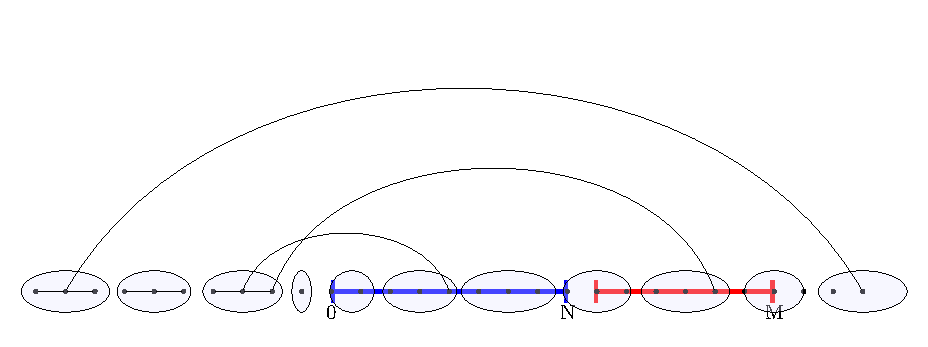
\includegraphics[page=1,width=0.9\textwidth]{fig.pdf}\]

The one-sided Ising model $\nu(x)$ is obtained from the random cluster model with respect
to spins in $V_+$ and the Bernoulli graph model of $\t^+$. 
We may write the marginal of the cylinder $\cy N$ for the \emph{one-sided Ising model} as
\[
  \nu(\cy N) =
  \frac{\XI{ 2^{\ol\omega_S(\t^+)} \cdot b(\t^+,\cy N)}}{\XI{2^{\omega(\t^+)}}}
  = \frac{\XI{ 2^{\ol\omega_S(\t^+) + f(\t')} \cdot b(\t^+,\cy N)}}{\XI{2^{\omega(\t^+)+f(\t')}}}.
\]
where $f(\t')$ denote any function of the graph $\t'$. 

\def\M{{M}}
\def\N{{N}}

Our aim is to show that for all $x\in\SI^{[0,\infty)}$
\[
  \lim_{M,L\to\infty} \frac{\mu(\cy \M \mid \cy \N)}{\nu(\cy\M \mid \cy\N)} = 1+\ordo N \quad\text{as $N\to\infty$.}
\]

From the computations above we deduce that 
\[
  \frac{\mu(\cy\N)}{\nu(\cy\N)} = \text{const.} \times
  \frac{\XI{2^{\ol\omega_\N(\t)} \cdot b(\t,\cy\N)}}
  {\XI{2^{\ol\omega_\N(\t^+) + f(\t')} \cdot b(\t^+,\cy\N)}}
\]
where the constant is \({\XI{2^{\omega(\t^+)}}}/{\XI{2^{\omega(\t)}}}\).


Then
\begin{equation}
  \ol\omega_N(\t) = \ol\omega_N(\t^+) + \ol\omega_N(\t^-) - X_N(\t') + Z_N(\t)
\end{equation}
where $X_N(\t')$ are the number of edges between clusters in $\mscr R^-_N$ and
$\ol N$. The term $Z_N(\t)$ is a correction term which is not independent of $\t^+$.
However, we have
\[ Z_N(\t) \le Y_N(\t')\]
where $Y_N(\t)$ is the number
\[
  Y_N(\t') = \sum_{C\in\mscr R^-_N} \max\{|E(C,\ol N)|-1,0\}
\]
We claim that $Y_N(\t')$ has distribution bounded by a Poisson variable
$\opn{Po}(\lambda_N)$ where $\lambda_N\to 0$ as $N\to\infty$. 

Similarly, we have for $0<N<M<L$ that
\[ b(\t,\cy M) = b(\t',\cy M) b(\t^+,\cy M)\cdot J(\t) \]
where $J(\t,\cy M)=0$ only if there is a component $C\in\mscr L^-$ such that
\[ |\t'(C,\ol N)| \ge 1 \quad\text{and}\quad |\t'(C,V_+)| \ge 2\]




\end{document}
